% *======================================================================*
%  Cactus Thorn template for ThornGuide documentation
%  Author: Ian Kelley
%  Date: Sun Jun 02, 2002
%  $Header: /home/eschnett/C/carpet/Carpet/Carpet/doc/documentation.tex,v 1.8 2003/07/16 10:49:09 hawke Exp $                                                             
%
%  Thorn documentation in the latex file doc/documentation.tex 
%  will be included in ThornGuides built with the Cactus make system.
%  The scripts employed by the make system automatically include 
%  pages about variables, parameters and scheduling parsed from the 
%  relevent thorn CCL files.
%  
%  This template contains guidelines which help to assure that your     
%  documentation will be correctly added to ThornGuides. More 
%  information is available in the Cactus UsersGuide.
%                                                    
%  Guidelines:
%   - Do not change anything before the line
%       % START CACTUS THORNGUIDE",
%     except for filling in the title, author, date etc. fields.
%        - Each of these fields should only be on ONE line.
%        - Author names should be sparated with a \\ or a comma
%   - You can define your own macros are OK, but they must appear after
%     the START CACTUS THORNGUIDE line, and do not redefine standard 
%     latex commands.
%   - To avoid name clashes with other thorns, 'labels', 'citations', 
%     'references', and 'image' names should conform to the following 
%     convention:          
%       ARRANGEMENT_THORN_LABEL
%     For example, an image wave.eps in the arrangement CactusWave and 
%     thorn WaveToyC should be renamed to CactusWave_WaveToyC_wave.eps
%   - Graphics should only be included using the graphix package. 
%     More specifically, with the "includegraphics" command. Do
%     not specify any graphic file extensions in your .tex file. This 
%     will allow us (later) to create a PDF version of the ThornGuide
%     via pdflatex. |
%   - References should be included with the latex "bibitem" command. 
%   - use \begin{abstract}...\end{abstract} instead of \abstract{...}
%   - For the benefit of our Perl scripts, and for future extensions, 
%     please use simple latex.     
%
% *======================================================================* 
% 
% Example of including a graphic image:
%    \begin{figure}[ht]
%       \begin{center}
%          \includegraphics[width=6cm]{MyArrangement_MyThorn_MyFigure}
%       \end{center}
%       \caption{Illustration of this and that}
%       \label{MyArrangement_MyThorn_MyLabel}
%    \end{figure}
%
% Example of using a label:
%   \label{MyArrangement_MyThorn_MyLabel}
%
% Example of a citation:
%    \cite{MyArrangement_MyThorn_Author99}
%
% Example of including a reference
%   \bibitem{MyArrangement_MyThorn_Author99}
%   {J. Author, {\em The Title of the Book, Journal, or periodical}, 1 (1999), 
%   1--16. {\tt http://www.nowhere.com/}}
%
% *======================================================================* 

% If you are using CVS use this line to give version information
% $Header: /home/eschnett/C/carpet/Carpet/Carpet/doc/documentation.tex,v 1.8 2003/07/16 10:49:09 hawke Exp $

\documentclass{article}

% Use the Cactus ThornGuide style file
% (Automatically used from Cactus distribution, if you have a 
%  thorn without the Cactus Flesh download this from the Cactus
%  homepage at www.cactuscode.org)
\usepackage{../../../doc/latex/cactus}
\usepackage{hyperref}

\begin{document}

% The author of the documentation
\author{Erik Schnetter \textless schnetter@uni-tuebingen.de\textgreater}

% The title of the document (not necessarily the name of the Thorn)
\title{Carpet}

% the date your document was last changed, if your document is in CVS, 
% please use:
\date{$ $Date: 2003/07/16 10:49:09 $ $}

\maketitle

% Do not delete next line
% START CACTUS THORNGUIDE

% Add all definitions used in this documentation here 
%   \def\mydef etc

% Add an abstract for this thorn's documentation
\begin{abstract}
This text describes the Carpet arrangement.  Carpet is a mesh
refinement driver for Cactus that can replace PUGH, the standard
unigrid driver.  Carpet supports multiple refinement levels and
multiple grid patches.  Carpet can run in parallel, but not yet very
efficiently so.  Carpet does not yet support multiple grid
hierarchies, i.e.\ shadow hierarchies or automatic convergence tests.
\end{abstract}



\section{Overview}

\subsection{Fixed Mesh Refinement, aka Box-in-Box}

Fixed Mesh Refinement (FMR), also known as box-in-box, is a way to
increase the local resolution in unigrid applications, while retaining
the basic unigrid character of an application.  A small number (maybe
two or three) of grids with varying resolution overlay each other,
where the coarsest grid has the largest extent.  This allows the
application to benefit from the higher resolution of the smaller grids
while keeping the outer boundary far out at the same time.  The main
advantage of FMR are that it needs far less resources than globally
increasing the resolution.

\subsection{Carpet}

Carpet is the name of an FMR driver, i.e.\ the back end that handles
storage allocation for the grid functions, parallelism, I/O, and the
various inter-grid operations.  Carpet was developed in early summer
of 2000 by Erik Schnetter \cite{Carpet__erik-schnetter}, then a
research scholar in the Department for Astronomy and Astrophysics
\cite{Carpet__astro-psu-edu} of Penn State University
\cite{Carpet__psu-edu}.  In spring 2001, Carpet was coupled to Cactus
as a drop-in enhancement for the standard unigrid Cactus driver PUGH.

\subsection{Cactus}

From the main Cactus web pages \cite{Carpet__cactuscode-org}:
\begin{quote}
Cactus is an open source problem solving environment designed for
scientests and engineers.  Its modular structure easily enables
parallel computation across different architectures and collaborative
code development between different groups.  Cactus originated in the
academic research community, where it was developed and used over many
years by a large international collaboration of physicists and
computational scientists.
\end{quote}



\section{Introduction}

\subsection{Fixed Mesh Refinement}

A standard way of solving partial differential equations are finite
differences on a regular grid.  This is also called \emph{unigrid}.
Such an application discretises its problem space onto a single,
rectangular grid which has everywhere the same grid spacing.  This
grid might be broken up into several parts for parallelisation
purposes, but parallelisation should be transparent to the physics
part of the application.

Increasing the resolution in a unigrid application is somewhat
expensive.  For example, increasing the resolution by a factor of two
requires a factor of eight more storage in three dimensions.  Given a
constant Courant factor, the calculation time will even go up by a
factor of sixteen.  This behaviour makes it easy to find problems that
cannot be solved on contemporary supercomputers, no matter how big and
fast those computers are.

Apart from physical insight, which often has to be used to decrease
the problem size until it fits the current hardware, there are also
numerical and algorithmic methods to decrease the resource
requirements of the application.  Most applications need the high
resolution only in a part of the simulation domain.  Discretisation
methods that don't require a uniform resolution, such as finite
elements, can implement non-uniform resolutions very naturally.  One
problem with finite elements is that many physicists today are not
familiar with finite elements, or shy away from their perceived
complexity, or are not willing to adapt existing finite difference
code.

Fixed Mesh Refinement (FMR) is a poor man's way of implementing a
non-uniform resolution into a unigrid application with minimal changes
to its structure.  Instead of only one grid, there are several grids
or grid patches with different resolutions.  The coarsest grid usually
encloses the whole simulation domain.  Successively finer grids
overlay the coarse grid at those locations where a higher resolutions
is needed.  The coarser grids provide boundary conditions to the finer
grid through interpolation.

Instead of updating only one grid, the application has to update all
grids.  The usual approach is to first take a step on the coarsest
grid, and then recursively take several smaller steps on the finer
grids.  The Courant criterion requires that the step sizes on the
finer grids be smaller than on the coarse grid.  The boundary values
for the finer grids are found through interpolation in space and time
from the coarser grid.  In the end, the information on the finer grids
is injected into the coarse grids.

Strictly speaking there is no need for a coarse grid on the regions
covered by the finer grids.  But as stated above, the resources
required for treating the overlapping region on the coarse grid are
only minimal compared to treating the finer grids.  And because a
coarse grid with a hole often creates complications, this obvious
optimisation is often left out.

\subsection{Carpet}

Carpet is a C++ library that provides infrastructure to describe
regions of varying resolution in a convenient and efficient way.
Carpet contains routines to manage grid hierarchies, containing the
relationships between the components of the grid on the different
refinement and convergence levels.  Carpet has a notion of simulation
time and grid spacing, which are necessary for interpolation, and
contains efficient interpolators.

Carpet can run on several processors in parallel using MPI for
communication.  Each grid can be broken down into several components,
and every component has a home processor.  Carpet also contains
operators to move certain regions to a different processor, or to
synchronise all components of a grid.

Carpet is also an arrangement of thorns for Cactus, implementing a
driver and associated I/O routines for both ASCII and binary I/O.  It
should be possible to substitute Carpet for the standard Cactus driver
PUGH without changes to the application thorns and thus use Carpet as
a unigrid driver.  Making use of the FMR capabilities of Carpet
usually requires some rearranging of the application, comparable in
general to the changes necessary for a uniprocessor application to run
on multiple processors.

The driver section of Carpet contains the logic to manage storage for
the grid functions, to traverse the grid hierarchy for all scheduled
routines, and to automatically apply the necessary inter-grid
operators for prolongation (interpolation of the fine grid boundaries)
and restriction (injecting the fine grid information back into the
coarse grid).

The ASCII I/O routines use the quasi-standard gnuplot
\cite{Carpet__gnuplot-info} format.  The binary I/O routines use the
FlexIO library \cite{Carpet__FlexIO} written by John Shalf.  It allows
efficient and platform independent I/O.  The FlexIO format is based on
HDF \cite{Carpet__HDF} and also supported by several visualisation
packages.

Carpet is copyrighted by Erik Schnetter, and is available under the
GPL licence from a CVS \cite{Carpet__CVS} repository.

\subsection{WaveToy}

Cactus comes with a sample application called \emph{WaveToy}, which
solves the scalar wave equation with various initial data and boundary
conditions.  An an example, I have extended WaveToy so that is uses
Carpet's FMR capabilities.  WaveToy serves both as a test case for
Carpet, and as example of how to convert an application to using FMR.

The equation solved by WaveToy is the well known scalar wave equation,
discretised using the Leapfrog method with three time levels, yielding
second order accuracy in space and time.  A typical set of initial
data are a plane wave, and a typical boundary condition is
periodicity.  Those allow long term simulations as well as easy and
meaningful comparisons to the analytic solution.



\section{Compiling Cactus With Carpet}

Carpet has been written in C++, using templates and the STL (Standard
Template Library).  Both templates and the STL make writing and
debugging code a lot easier.  Without templates, I would have had to
put much effort into making Carpet support all of Cactus' data types.
Without the STL, I would have had to spend quite some time
implementing basic containers such as lists or sets.  I still had to
implement a custom vector type, because STL's vector type is optimised
for large vectors only, and I needed threedimensional vectors of
integers.

The inner loops of Carpet are the inter-grid operators, that is the
routines that copy, restrict, and prolongate between grids.  Due to
Cactus it was rather easy to write these in \textsc{Fortran 77}, which
makes them both fast and portable.

Carpet is an arrangement in Cactus.  It can theoretically be compiled
without any other external library, if you don't include the binary
I/O support which requires FlexIO.  I do recommend using FlexIO, so
you should install the FlexIO library first.  Although FlexIO is
already part of Cactus in the thorn called CactusExternal/FlexIO, this
seems to be a version that has FMR support disabled and is hence not
usable.  You will have to install a complete copy of FlexIO by hand.

\subsection{Hurdle 1: FlexIO}

I suggest that you enable support for the HDF format in the FlexIO
library, although this is not necessary.  If you don't want to do
this, then you don't have to install the HDF libraries in the
following.

\begin{enumerate}

\item
Install the HDF4 and HDF5 libraries.  They are available from the HDF
web pages \cite{Carpet__HDF}, and they can be installed with the usual
\texttt{./configure; make; make install} triplet.  They should already
be installed by default on most machines.  The conversion utilities
between HDF4 and HDF5 are installed automatically when you install
HDF5 while HDF4 is already installed.  (That means that you should
install HDF4 first, and then HDF5.)

\item
Get the FlexIO library from the Cactus CVS server:\\ \texttt{cvs -d
:pserver:\textit{yourlogin}@cvs.cactuscode.org:/packages checkout
FlexIO}.  If you do not have a login, then use the login
\texttt{cvs\_anon} for anonymous access.  The Cactus web pages
describe how to do this.

\item
Configure FlexIO while providing the paths to the HDF4 and HDF5
libraries: \texttt{./configure --with-hdf4=/usr --with-hdf5=/usr},
assuming that HDF4 and HDF5 are installed under \texttt{/usr}.  You
can also configure without HDF support, but then you will not be able
to read or write HDF files.  FlexIO will then support only the
built-in \texttt{IEEEIO} format.

\item
Edit the top of the file \texttt{FlexIO/Makefile} to match your actual
configuration.  The \texttt{./configure} script of FlexIO is a bit
simplistic, so don't spend too much effort trying to convince it to do
the right thing.

On my machine, I had to change the settings \texttt{CC = mpicc},
\texttt{C++ = mpiCC -DMPICH\_SKIP\_MPICXX}, and \texttt{HDFINCLUDES =
-I\$(HDFROOT)/include/hdf} by hand.  I am using Debian Linux on an
IA32 with gcc 2.95.4 and MPICH 1.2.4, and I have an HDF5 library where
support for parallel I/O was enabled.

\item
Compile the library with \texttt{make}.

\item
The library cannot be installed automatically.  You usually use the
include and library files where they are.  If you want to install the
library, copy all the header files (\texttt{*.h *.hh *.H}) and the
library files (\texttt{*.a}).

\end{enumerate}

Yes, I also think that this is way too complicated.

\subsection{Hurdle 2: STL}

Some operating systems do not have a compliant STL (Standard Template
Library) installed.  If not, then you are in trouble.  Carpet does
make use of the STL, and there is no way around that.

\subsection{Hurdle 3: Templates}

Some compilers contain switches to instantiate some or all templates
automatically.  This usually does not work when files are put into
libraries, which is what Cactus does.  The scheme that I found working
on all machines is to instantiate most templates by hand, and have the
compiler instantiate the missing templates for every object file.
This is the default for gcc.  On SGIs, you have to pass the options
\texttt{-no\_auto\_include -ptused} to the C++ compiler.

The C++ standard specifies a limit when using templates as template
parameters.  Carpet's use of the GNU STL exceeds this limit.  Gcc
requires the option \texttt{-ftemplate-depth-30} to enable this.

\subsection{WaveToy}

Unfortunately, PUGH and Carpet cannot yet be both compiled into a
single application.  (This will be fixed soon.)  That means that you
will have separate executables for unigrid and for mesh refinement
applications.

Configuring Carpet is not quite trivial, because Cactus provides
currently no way to autodetect the settings for Carpet.  Hence you
will have to set the settings manually.  I propose that you start with
on of the pre-made options files in the directory
\texttt{Carpet/Carpet/options}.  Try e.g.\ \texttt{carpet-harpo-sgi}
for an SGI, or \texttt{carpet-lilypond} for Linux with gcc, or
\texttt{carpet-lilypond-ic} for Linux with the Intel compilers.  Once
you have a working options file for your machine, send it to me, so
that I can include it.

As for the thorn list: Carpet has its own ASCII output thorn, which
outputs more information than CactusBase/IOASCII.  The thorn list that
I use is

\begin{verbatim}
CactusBase/Boundary                # boundary (grid) [ ] { }
CactusBase/CartGrid3D              # grid ( ) [ ] {driver}
#CactusBase/IOASCII                 # IOASCII (IO,Hyperslab) [ ] {IO}
CactusBase/IOBasic                 # IOBasic (IO) [ ] {IO}
CactusBase/IOUtil                  # IO ( ) [ ] { }
CactusBase/LocalInterp             # LocalInterp ( ) [ ] { }
CactusBase/Time                    # time ( ) [ ] { }
CactusConnect/HTTPD                # HTTPD (Socket) [ ] {Cactus}
CactusConnect/HTTPDExtra           # http_utils (httpd,IO) [ ] { }
CactusConnect/Socket               # Socket ( ) [ ] { }
#CactusExternal/FlexIO              # FlexIO ( ) [ ] { }
CactusExternal/jpeg6b              # jpeg6b ( ) [ ] { }
CactusIO/IOJpeg                    # IOJpeg (IO,Hyperslab,jpeg6b) [ ] {IO}
CactusUtils/NaNChecker             # NaNChecker ( ) [ ] { }
CactusWave/IDScalarWave            # idscalarwave (wavetoy,grid) [ ] {grid}
CactusWave/IDScalarWaveC           # idscalarwave (wavetoy,grid) [ ] {grid}
CactusWave/IDScalarWaveCXX         # idscalarwave (wavetoy,grid) [ ] {grid}
#CactusWave/IDScalarWaveElliptic    # idscalarwaveelliptic (grid,wavetoy,ellbase) [ ] {idscalarwave}
CactusWave/WaveBinarySource        # binarysource (wavetoy,grid,idscalarwave) [ ] { }
CactusWave/WaveToyC                # wavetoy (Grid,Boundary) [ ] { }
CactusWave/WaveToyCXX              # wavetoy (Grid,Boundary) [ ] { }
CactusWave/WaveToyF77              # wavetoy (Grid,Boundary) [ ] { }
#CactusWave/WaveToyF90              # wavetoy (Grid,Boundary) [ ] { }
#CactusWave/WaveToyFreeF90          # wavetoy (Grid,Boundary) [ ] { }
Carpet/Carpet                      # driver (CarpetLib) [ ] {Cactus,IO}
Carpet/CarpetIOASCII               # IOASCII (CarpetLib,driver,Hyperslab) [ ] {IO}
Carpet/CarpetIOFlexIO              # IOFlexIO (CarpetLib,driver,Hyperslab) [ ] {IO}
#Carpet/CarpetIOHDF5                # IOHDF5 (CarpetLib,driver,Hyperslab) [ ] {IO}
#Carpet/CarpetIOSer                 # IOSer (CarpetLib,driver,Hyperslab) [ ] {IO}
Carpet/CarpetLib                   # CarpetLib ( ) [ ] { }
Carpet/CarpetReduce                # reduce (CarpetLib,driver) [ ] { }
Carpet/CarpetRegrid                # CarpetRegrid (CarpetLib,driver) [ ] { }
Carpet/CarpetSlab                  # Hyperslab (CarpetLib,driver) [ ] { }
\end{verbatim}

The thorns prefixed with \texttt{\#} are disabled.  IOASCII conflicts
with CarpetIOASCII, and FlexIO conflicts with the external FlexIO
library that CarpetIOFlexIO uses.  I disabled IDScalarWaveElliptic
because there is no elliptic solver for mesh refinement, and I
disabled WaveToyF90 and WaveToyFreeF90 because gcc does not contain a
Fortran 90 compiler.  CarpetIOHDF5 is not yet finished, and
CarpetIOSer needs the Ser library which is not publically available.

The CactusConnect, CactusExternal, CactusIO, and CactusUtils thorns
are not necessary, but are nice to have around.  You can safely omit
these.



\section{Running The Example Applications}

Although Carpet works fine with the standard WaveToy thorns, all the
example parameter files in the CactusWave arrangement use PUGH, and
can therefore not be directly used.

The coordinate thorn CactusBase/CartGrid3D does not provide periodic
boundary conditions.  These are normally provided by the driver PUGH.
However, Carpet does not contain any boundary conditions.  If you want
to apply periodic boundaries, you will therefore have to use the
AlphaThorns/Cart3d coordinate thorn instead, which does provide
periodicity.  Unfortunately, AlphaThorns/Cart3d is incompatible with
CactusBase/CartGrid3D.  There is a version of WaveToy in the Carpet
arrangement that has been adapted to AlphaThorns/Cart3d.  I suggest
that you use this version of WaveToy instead of CactusWave to run test
problems, because periodicity makes for nice testing setups.

You can find quite a few example parameter files in the directory
\texttt{Carpet/WaveToyF77/par}.  I especially recommend the
\texttt{wavetoyf77\_periodic\_*} set, which comes in two sizes
(\texttt{coarse} and \texttt{fine}, corresponding to a small and a
large simulation domain) and three different refinement hierarchies
(with one, two, and three level altogether, respectively).  This set
thus forms a convergence test, which you can run and test yourself.
The set \texttt{wavetoyf77\_rad\_full\_*} uses radiative instead of
periodic boundaries and should also be nice to look at.  The file
\texttt{wavetoyf77\_rad\_automatic.par} is an attempt at adaptive mesh
refinement, which may or may not work, depending on the current status
of Carpet.

Second order convergence requires second order interpolation in time,
which requires that at least three time levels are present.



\section{Fold Your Own FMR Application}

There are three steps to take from a simple unigrid uniprocessor toy
application to a full-blown FMR multiprocessor production application.
Those steps are almost independent, and I would like to explain them
and their implications in some detail below.

\subsection{Multiple Processors}

The probably best known of these is the step from using one to using
several processors, also known as parallelisation.  Because many
people are already familiar with this step, I will describe it first.

In a uniprocessor application, it is possible to access every grid
point in arbitrary manners.  In order to allow multiple processors to
run efficiently in parallel, the grid is broken down into several
rectangular components, and each processor is assigned one of these
components.

The components will usually overlap by a few grid points, so as to
allow the processors to e.g.\ calculate spatial derivatives (which
require neighbouring grid points) without having to communicate for
every grid point.  From time to time it is then necessary to
synchronise the overlapping region, which is the only time at which
communication happens.  This allows the application to run almost
unchanged, i.e.\ without invoking communication itself.  The
synchronisation routine is provided by the driver and not by the
application.

Of course a serial applicate usually will have to be changed to
support multiple processors.  In order to do so, all the operations
that the application performs have to be classified into one of two
categories:

One category contains the so-called \emph{local} operations.  These
are operations that are applied to each and every grid point
individually, and that do not depend on any other grid point except
nearby neighbours.  Each local operation will thus involve a loop over
all grid points, and in order to run on multiple processors, after
each such loop the synchronisation routine has to be called.  An
example of a local operation would be calculating a spatial
derivative.

The other category contains so-called \emph{global} operations.  These
operations do not depend on individual grid points, and thus do not
involve loops over grid points.  The result of a global operation is
the same on all processors; therefore global operations don't involve
communication and don't require synchronisation.  An example of a
global operation would be to check how many time steps have been
taken, and decide whether the simulation should be terminated.

Typically most operations can be classified or rewritten to be either
local or global.  But often there are operations that fit neither
category, and these parts of an application are hardest to
parallelise.  Applying the boundary conditions, to give another
example, might seem at first to be neither local nor global.  But in a
slight (yet completely correct) stretch of the term "applied to all
grid points", boundary conditions can be classified as local; they are
a local operation that just does nothing to most grid points.

To give one more example, calculating an error norm does not fit these
categories.  It is neither local nor global.  It is not local because
the results involved all grid points (and not only nearby neighbours),
and it is not global because it does involve the grid points.  All
operations that do not fit the two category require typically special
handling, and often require hand-coded communication in the
application.  Luckily calculating various norms is such a common case
that there are special routines for that already present, called
\emph{reduction operators}.

\subsection{Multiple Resolution Levels}

There are several reasons why an application might want to incorporate
more than one grid, overlapping and each with a different resolution.

The most commonly known reason is probably a convergence test, where
the very same problem is treated in different resolutions.
Differences in the result are then likely caused by insufficient
resolution on the coarser (or on all) grids.  For a convergence test,
the grids are completely independent, and it does not matter whether
the simulation runs on all grids simultaneously or sequentially.  In
order to treat the grid sequentially, the application does not have to
be changed at all.

The reason of interest here is of course FMR.  For FMR, the order in
which the grids are treated is fixed.  As described above, there is
first a time step on the coarse grid, and then recursively several
smaller steps on the finer grids.  This order does require certain
changes in the application.  The sequence of operations that form a
single time step have to be identified and isolated.  (Which is to say
that there has to be a routine that calculates a time step, that is, a
complete time step, and nothing else.)  It is then the task of the FMR
driver to call this routine for the correct grids in the correct
order.

Other reasons for multiple resolution levels are e.g.\ multigrid
algorithms for elliptic equations, which I do not want to mention
here, or shadow hierarchies to determine truncation errors, which I
also want to skip here.  Shadow hierarchies are very similar to the
convergence levels described above.

Apart from this order in which the operations are performed on the
grids, there is one more complication for FMR.  The boundary values of
the finer grids have to be calculated from the coarser grids through
interpolation.  An because the time steps on the finer grids are
smaller, there is not always a corresponding value on the coarser
grids available.  This makes it necessary to interpolate in time
between time steps on the coarser grids.  The alternative would be to
take smaller steps on the coarser grids, and this would be very
expensive.

These interpolations in time make it necessary that the driver knows
which grid function contains values corresponding to what time.  The
usual way to achieve this is to have several time levels per grid
function; three time levels allow for a second order interpolation in
time.  Only grid functions with enough time levels can be
interpolated, i.e.\ boundary conditions can be calculated only for
those.

Fortunately time levels are rather widespread in applications, so they
are no new concept to introduce.  Unfortunately they are often abused,
so that values corresponding to the wrong time are stored in a time
level, usually with the excuse of saving storage.  This will in
general not work with FMR, because the driver then cannot interpolate
in time, leading to incorrect values on the boundaries of the finer
grids.

\subsection{Multiple Grid Components}

Sometimes it is convenient to have a simulation domain that is not a
rectangle.  It might instead be an L-shaped simulation domain, or a
domain that consists of two disconnected rectangular regions.  This
issue becomes more important with FMR, because there it is often
convenient to have several disconnected refined regions.  As long as
there are enough processors available, each processor can be assigned
a region or a part thereof, and no new concept need be introduced.
If, however, there are fewer processors than regions, then a new
problem arises.

A common case for that problem might be a simulation containing just
two refined regions, and running on a single processor.  The refined
grid the consists of two component.  The problem then is that the two
components cannot be treated sequentially: Imagine the time evolution
routine working on (say) the first component.  It will at some time
call the synchronisation routine.  At that time there are no values
from the second component available, because the second component has
not been treated yet.  Therefore the synchronisation routine cannot
complete.  That means in turn that the time evolution routine cannot
complete working on the first component, leading to a deadlock.  Work
on neither component can be completed before work on the other
component.

The solution is to break up the time evolution routine into several
smaller routines, each consisting of a single either local or global
operation.  (``Local'' and ``global'' have here the exact same
meanings that were defined above for parallelisation.)  A local
operation works, by definition, on individual grid points.  Hence the
local routines have to be called once for every grid component.  A
global operation, by definition, does not depend on individual grid
points.  Hence it has to be called only once per processor, and not
once per component.  That means that the driver has to be told the
category individual routine is in.

\subsection{Example}

Let me finish this section with an detailed example.  Suppose you want
to solve the equation
\begin{eqnarray}
   \frac{d}{dt} u & = & f(u) \quad ,
\end{eqnarray}
integrating using the midpoint rule, i.e.\ the simplemost second-order
time integration scheme.  Given values at the previous time $u^{n-1}$,
one first calculates a first order solution using an Euler step,
leading to the intermediate result
\begin{eqnarray}
   v^n & = & u^{n-1} + dt\; f(u^{n-1}) \quad .
\end{eqnarray}
The second and final step is then calculated via
\begin{eqnarray}  
   u^n & = & u^{n-1} + dt\; f(\frac{1}{2} [u^{n-1} + v^n]) \quad .
\end{eqnarray}

The corresponding pseudo code would look like
\begin{enumerate}
\item
Calculate Euler step, storing the result into $u^n$
\item  
Apply boundary conditions to $u^n$
\item  
Synchronise $u^n$
\item  
Calculate average of $u^{n-1}$ and $u^n$, storing the result into
$v^n$
\item  
Calculate second step, storing the result again into $u^n$
\item
Apply boundary conditions again to $u^n$
\item  
Synchronise again $u^n$
\end{enumerate}

The above algorithm looks a bit different from a naive implementation
of the midpoint rule.  One difference is that both the first and the
second step store their result into $u^n$.  This is necessary because
it would be inconvenient to apply boundary conditions to the
intermediate value $v^n$.  Remember, in order to apply boundary
conditions on the finer grids, there have to be several time levels
present.  With the above scheme, only $u$ needs several time levels.
$v$ is used only as a temporary (and could conceivably be completely
eliminated).

Note also that the first step goes all the way from time level $n-1$
to time level $n$.  The midpoint rule can be rewritten (in fact, is
usually written) so that the first step is only a half step, leading
to the time level $n - \frac{1}{2}$.  This is not possible for FMR,
because interpolating to the time $n - \frac{1}{2}$ is not possible,
and thus there could be no boundary conditions applied after the first
step.

The second thing to note is that the application of the boundary
condition and the synchronisation have been separated rather
artificially.  Normally synchronisation would be considered part of
the boundary condition.  In this case, however, the applying the
boundary condition is a local operation, whereas synchronisation
counts as global operation.  (It is not obvious that synchronisation
should be global, but as the synchronisation routine is a part of
Carpet, it was up to me to decide this.)  As explained above, local
and global operations have to be separated.

Separating the evolution steps and the boundary condition routines is,
on the other hand, just a notational convenience.  There could well be
a single routine implementing both.

For Cactus, the order in which to call the individual parts of the
time evolution routines is described in the schedule routines, i.e.\
in the files called \texttt{schedule.ccl}.  By default a routine is
assumed to be local; global routines have to be tagged with
\texttt{OPTIONS: GLOBAL}.

The tag \texttt{SYNC: groupname} indicates that the group
\texttt{groupname} should be synchronised after the scheduled routine
has been called for all grid components.  This obviously makes sense
only for local routines.  Using the \texttt{SYNC:} tag is preferred
over calling the synchronisation routine \texttt{CCTK\_SyncGroup}
directly.

The example thorn WaveToy in Carpet's arrangement is a bit simpler
than what is described here, because it uses the Leapfrog scheme which
consists of only a single step.  I would suggest looking at WaveToy as
an initial FMR example.

The thorn SpaceToy is implemented very close to the way described
here.  It evolves two variables phi and psi, but it is also coupled to
the thorn HydroToy.  This coupling introduces some additional
complications.  The thorn HydroToy, on the other hand uses a
predictor-corrector scheme, which is also a two step scheme and thus
more complex that WaveToy.  All the coupling between SpaceToy and
HydroToy is contained in SpaceToy.  I would thus suggest looking at
HydroToy first.

I assume that converting an application to FMR is straightforward
after handling the time levels has been straightened out.



\section{Further documentation}

The individual thorns in the Carpet arrangement might contain further
documentation, which is also available in the thorn guide.
Additionally, there is a document \texttt{internals.tex} in the
arrangement's doc directory, and a document
\texttt{threelev\_initdata.tex} in thorn \texttt{Carpet}'s doc
directory.


\section{Frequently Asked Questions}
\label{sec:faq}

Here are a few of the more frequently asked questions with some
answers.
\begin{enumerate}
\item \textbf{If I run without any refined grids, why don't I get the
    same results as with PUGH?}
  
  There are two possible reasons. The most common is that the you are
  not comparing exactly the same output. It used to be the case that
  norms would disagree (this is no longer the case). If it is the
  ASCII output that disagress, then you should note that the default
  output format for CarpetIOASCII gives more digits than
  CactusBase/IOASCII. If you want to get ``identical'' results for
  this output, try setting \texttt{IOASCII::out\_format = ".14f"}).

  The second reason is subtle differences are bugs in the
  implementation. Good luck finding these...
\item \textbf{I switch on a refined grid. Why do I not see it output?
    Why is the output strange?} 

\begin{figure}[htbp]
  \begin{center}
    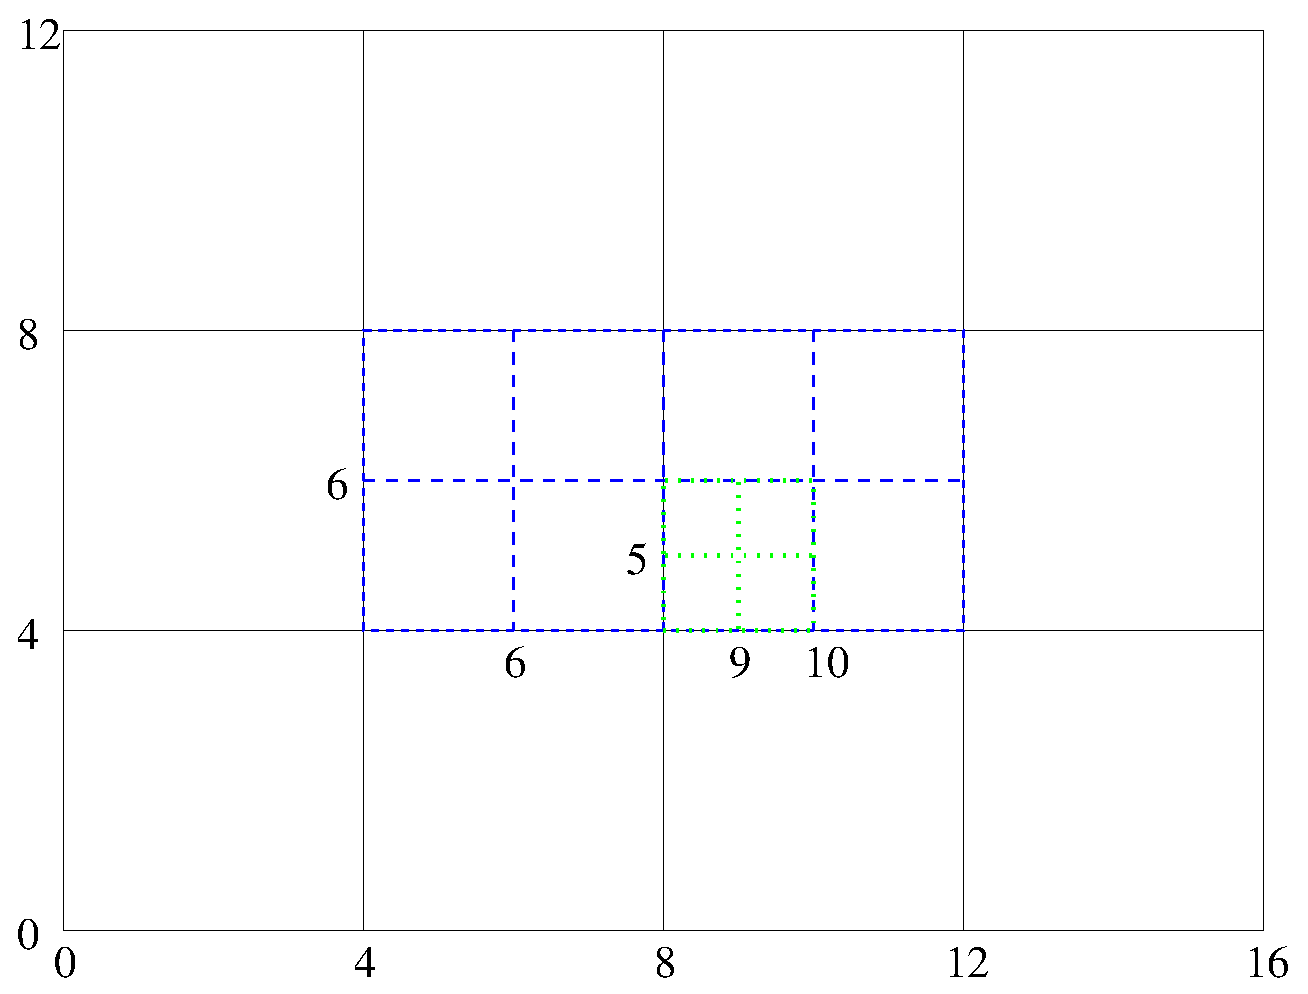
\includegraphics[scale=0.5]{Grid1.eps}
    \caption{How the grids are indexed in Carpet. This is an
      artificial three level example using C-style numbering (0
      origin). Note that the numbering is with respect to the finest
      grid.}
    \label{fig:Grid1}
  \end{center}
\end{figure}
  As soon as you switch on refinement the way the grids are numbered
  by index changes. The numbering is done with respect to the
  \textit{finest} grid but covers the entire domain. An example of how
  the numbering works is given in figure~\ref{fig:Grid1}. It is
  important to note that this also applies to the numbering in
  time. So with the grid structure of figure~\ref{fig:Grid1} output
  for the coarsest grid only occurs on iterations $0,4,8,\dots$, for
  the medium grid only on iterations $0,2,4,\dots$, and for the finest
  grid on iterations $0,1,2,\dots$. Note that here the finest grid is
  not the finest \textit{existing} grid, but the finest
  \textit{possible} grid. This is controlled by the
  \texttt{Carpet::max\_refinement\_levels} parameter.

  So, there are plenty of reasons why the output might be strange:
  \begin{itemize}
  \item You are requesting output on iterations when not all grids are
    output. For example, requesting output every $5^{\text{}th}$
    iteration with the above grid structure would only output the
    coarse grid every 20 iterations.
  \item You are requesting output along an index that does not
    intersect with any grid points. For example, the line defined by
    $j = 6$ in the example above corresponds to the center of the box,
    but does not intersect the coarse grid at all!
  \item Requesting output along a line defined by a coordinate value
    will give you the index closest to it. This may not agree on the
    different refinement levels. In the example above the coordinate
    value $y=5.1$ is closest to $j=5$ on the fine grid, $j=6$ on the
    medium grid, and $j=4$ on the coarse grid. All the different lines
    will be output but you should not expect points that appear to
    overlap in the output to agree as they're actually not at the same
    point. 
  \item CarpetRegrid (which sets up the refined boxes) knows nothing
    about symmetries. So if you have a simulation in, for example,
    octant mode with $x,y,z\in[0,10]$ and you leave all the parameters
    to be the defaults, the following will happen:
    \begin{itemize}
    \item CarpetRegrid creates a refined box at the center of the
      \textit{index space}. This might cover something like
      $x,y,z\in[3,7]$. 
    \item When the IO thorn requests the output lines and planes it
      does know the symmetries, so tries to put the lines and planes
      as close to the origin $x=y=z=0$ as possible.
    \item When output occurs the lines and planes don't intersect the
      fine grid and so you get no output.
    \end{itemize}
  \end{itemize}
  
  Morals: Comparing 1D output on different refinement levels can be
  very frustrating. 2D output is usually much more informative. Using
  symmetry conditions with Carpet is tricky.

\item {\bf I want to run with periodic boundaries. Why aren't things
    working correctly?}

  You thought symmetry boundaries were bad? Periodic boundaries are
  even worse.

  Firstly, Carpet does not itself implement periodic boundaries. The
  thorn {\tt TAT/Periodic} is ``more or less'' driver independent and
  does. This should be used to implement the actual boundary
  conditions. You should not need to change your code - just activate
  the thorn with the appropriate parameters.

  Secondly, periodic boundaries do {\bf not} work the same way as
  symmetry boundaries. This is because you cannot specify a point in
  coordinate space where the boundary actually lies; it really lies in
  the index space. The following example will hopefully help.
  
  Take a 1D slice through the grid. There are 7 points with 2 boundary
  (ghost) zones (0,2 and 10,12), so only 3 points are actually being
  evolved (4, 6, 8). Periodic boundaries means that the boundary points
  are identified with certain evolved points. For example, point 2 is
  to the left of the first evolved point and so must be identified
  with the \textit{last} evolved point (8). The identifications are
  shown in figure~\ref{fig:Periodic1}.
  \begin{figure}[htbp]
    \begin{center}
      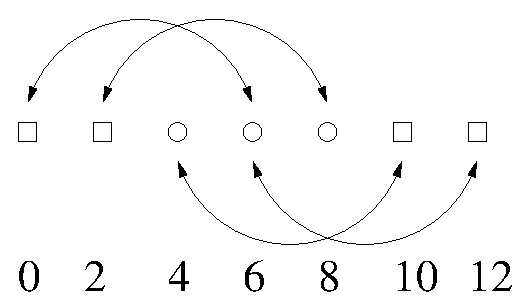
\includegraphics[scale=0.5]{Periodic1.eps}
      \caption{Periodic grids identify boundary points and interior
        points. The interior points are given by circles and the
        boundary points by squares. The identifications are shown by the
        arrows.}
      \label{fig:Periodic1}
    \end{center}
  \end{figure}

  We then want to place a refined region across the entire width of
  the domain but also have the correct periodic boundaries. The
  crucial point is to ensure that points that are identified on the
  coarse grid are identified in the same way on the fine grid. For
  example, point 2 must still be identified with point 8. Therefore
  point 2 must remain a boundary point and point 8 an interior
  point. Point 4 must also be identified with point 10. There are
  therefore 2 possibilities:
  \begin{itemize}
  \item Point 3 is the first interior point on the refined grid and
    point 8 the last. Therefore the point to the ``left'' of point 3,
    point 2, is still identified with point 8.
  \item Point 4 is the first interior point on the refined grid and
    point 9 the last. This possibility is illustrated in
    figure~\ref{fig:Periodic2}.
  \end{itemize}
  \begin{figure}[htbp]
    \begin{center}
      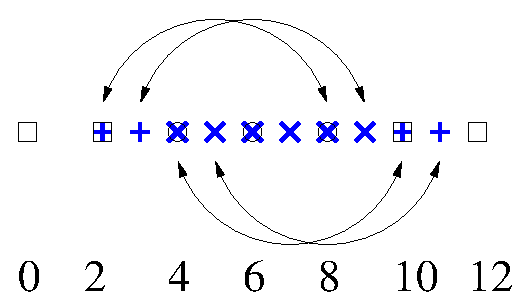
\includegraphics[scale=0.5]{Periodic2.eps}
      \caption{A periodic refined grid. The boundary zones are blue
        plus signs, the interior blue crosses. Note that the interior
        points on the refined grid extend \textit{outside} the
        interior on the base grid. However, equivalent points on both
        grids coincide.}
      \label{fig:Periodic2}
    \end{center}
  \end{figure}
  
  So to specify the particular refined grid shown in
  figure~\ref{fig:Periodic2} you would specify a lower bound of 2, an
  upper bound of 11, and that both boundaries are outer boundaries. An
  example for a $44 \times 7 \times 7$ grid where the ``centre half''
  of the grid in the $x$ direction is refined and the refined region
  covers the entirety of the $y$ and $z$ directions, you could use
\begin{verbatim}
carpet::max_refinement_levels   = 2
carpetregrid::refinement_levels = 2
carpetregrid::refined_regions   = "manual-gridpoint-list"
carpetregrid::gridpoints        = "[ [ ([22,2,2]:[62,11,11]:[1,1,1]) ] ]"
carpetregrid::outerbounds       = "[ [ [[0,0],[1,1],[1,1]] ] ]"
\end{verbatim}

\end{enumerate}

%% \bibliographystyle{amsalpha}      % initials + year
%% \bibliography{carpet}

\providecommand{\bysame}{\leavevmode\hbox to3em{\hrulefill}\thinspace}
\providecommand{\MR}{\relax\ifhmode\unskip\space\fi MR }
% \MRhref is called by the amsart/book/proc definition of \MR.
\providecommand{\MRhref}[2]{%
  \href{http://www.ams.org/mathscinet-getitem?mr=#1}{#2} }
\providecommand{\href}[2]{#2}
\begin{thebibliography}{{Pen}}

\bibitem[AA]{Carpet__astro-psu-edu}
{Department for} Astronomy and Astrophysics,
  \emph{\href{http://www.astro.psu.edu/} {http://www.astro.psu.edu/}}.

\bibitem[{Cac}]{Carpet__cactuscode-org}
{Cactus web pages}, \emph{\href{http://www.cactuscode.org/}
  {http://www.cactuscode.org/}}.

\bibitem[CVS]{Carpet__CVS}
CVS, \emph{\href{http://www.cvshome.org/} {http://www.cvshome.org/}}.

\bibitem[gnu]{Carpet__gnuplot-info}
gnuplot, \emph{\href{http://www.gnuplot.info/} {http://www.gnuplot.info/}}.

\bibitem[HDF]{Carpet__HDF}
HDF, \emph{\href{http://hdf.ncsa.uiuc.edu/} {http://hdf.ncsa.uiuc.edu/}}.

\bibitem[{Pen}]{Carpet__psu-edu}
{Penn State University}, \emph{\href{http://www.psu.edu/}
  {http://www.psu.edu/}}.

\bibitem[Sch]{Carpet__erik-schnetter}
Erik Schnetter, \emph{\href{mailto:schnetter@uni-tuebingen.de} {\textless
  schnetter@uni-tuebingen.de\textgreater}}.

\bibitem[Sha]{Carpet__FlexIO}
John Shalf, \emph{{FlexIO} library:
  \href{http://zeus.ncsa.uiuc.edu/~jshalf/FlexIO/}
  {http://zeus.ncsa.uiuc.edu/\textasciitilde jshalf/FlexIO/}}.

\bibitem[TAT]{Carpet__tat-physik-uni-tuebingen-de}
Theoretische Astrophysik T\"ubingen,
  \emph{\href{http://www.tat.physik.uni-tuebingen.de/} {http://www.tat.physik.uni-tuebingen.de/}}.

\end{thebibliography}

% Do not delete next line
% END CACTUS THORNGUIDE

\end{document}
